% !TEX root = DesignDocument.tex


\chapter{Overview and concept of operations}

The purpose of this project is to develop a virtual reality environment that accurately represents the Ruth Brennan art exhibit at the Dahl Arts Center.  The end product will be able to be transported to and from the museum too allow students and others, who otherwise cannot visit the museum, to experience the Dahl.

The end goal for this particular project is to have the prototype gallery running using the Oculus Rift and Unreal Engine.  This is so the Dahl Arts Center can get an accurate grasp of how this sort of technology will work and will inform their decision about whether to go further with the Oculus or not.  This leads to another goal for the project team, research additional methods to utilize the virtual reality of the Oculus and give the Dahl a better understanding of what is feasible and what is fantasy.

The system that is going to be used for this project uses the Unreal Engine for the environment and the Oculus Rift for the virtual reality immersion.  In order to allow users to experience this virtual gallery, there will have to be an operator who will know how to setup the Oculus and Unreal Engine for the tour to run efficiently.  

\section{Team Members and Team Name}
The team for this project, Virtual Dahl Art Gallary, consists of Alex Nienhueser and Mackenzie Smith. 

% !TEX root = SystemTemplate.tex


\section{Resumes}

%Your resumes are included here.  See the source file (industrial.tex) and uncomment the PDF includes to see how this works.  If your resume is written in \LaTeX\ then you can just insert the \LaTeX\ source code.

    \includepdf[pages={1}]{report.pdf}  %% example of limited page include

	  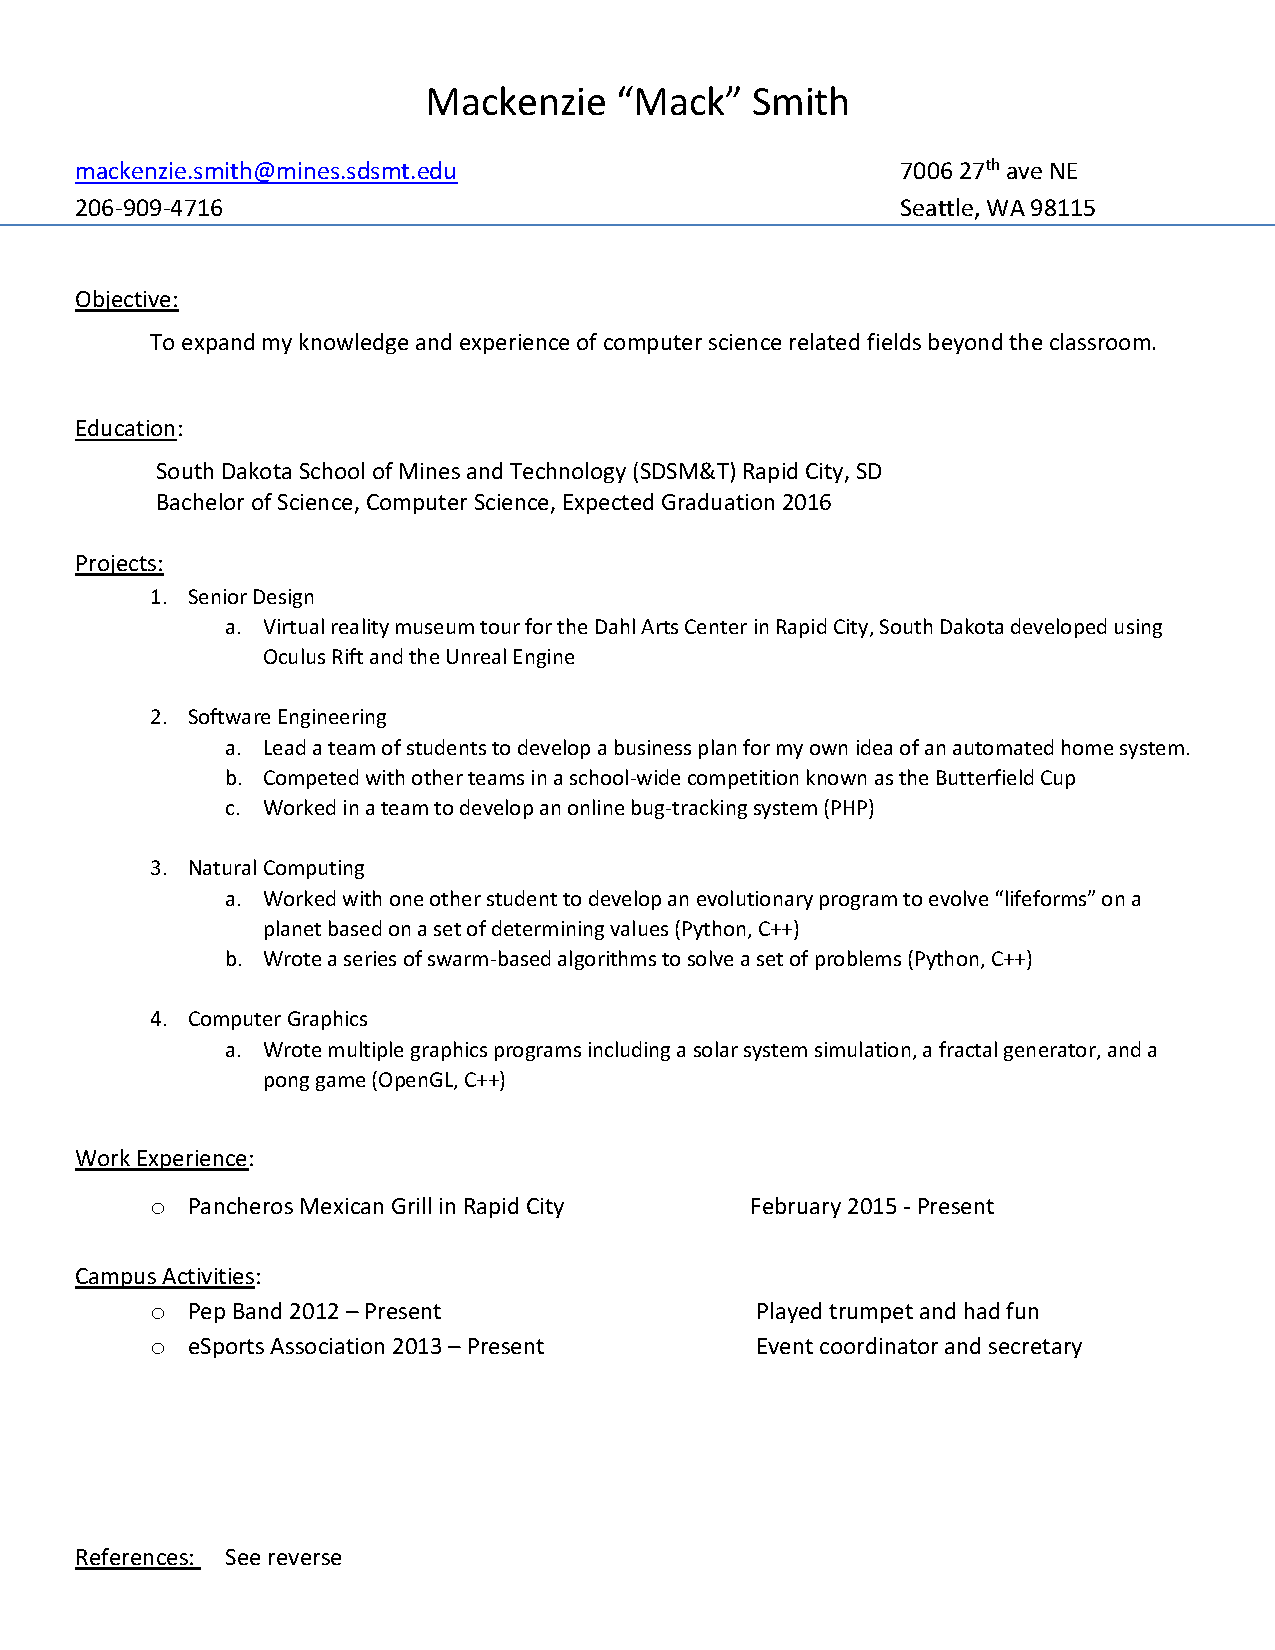
\includepdf{Resumes/Mack'sResume.pdf}
      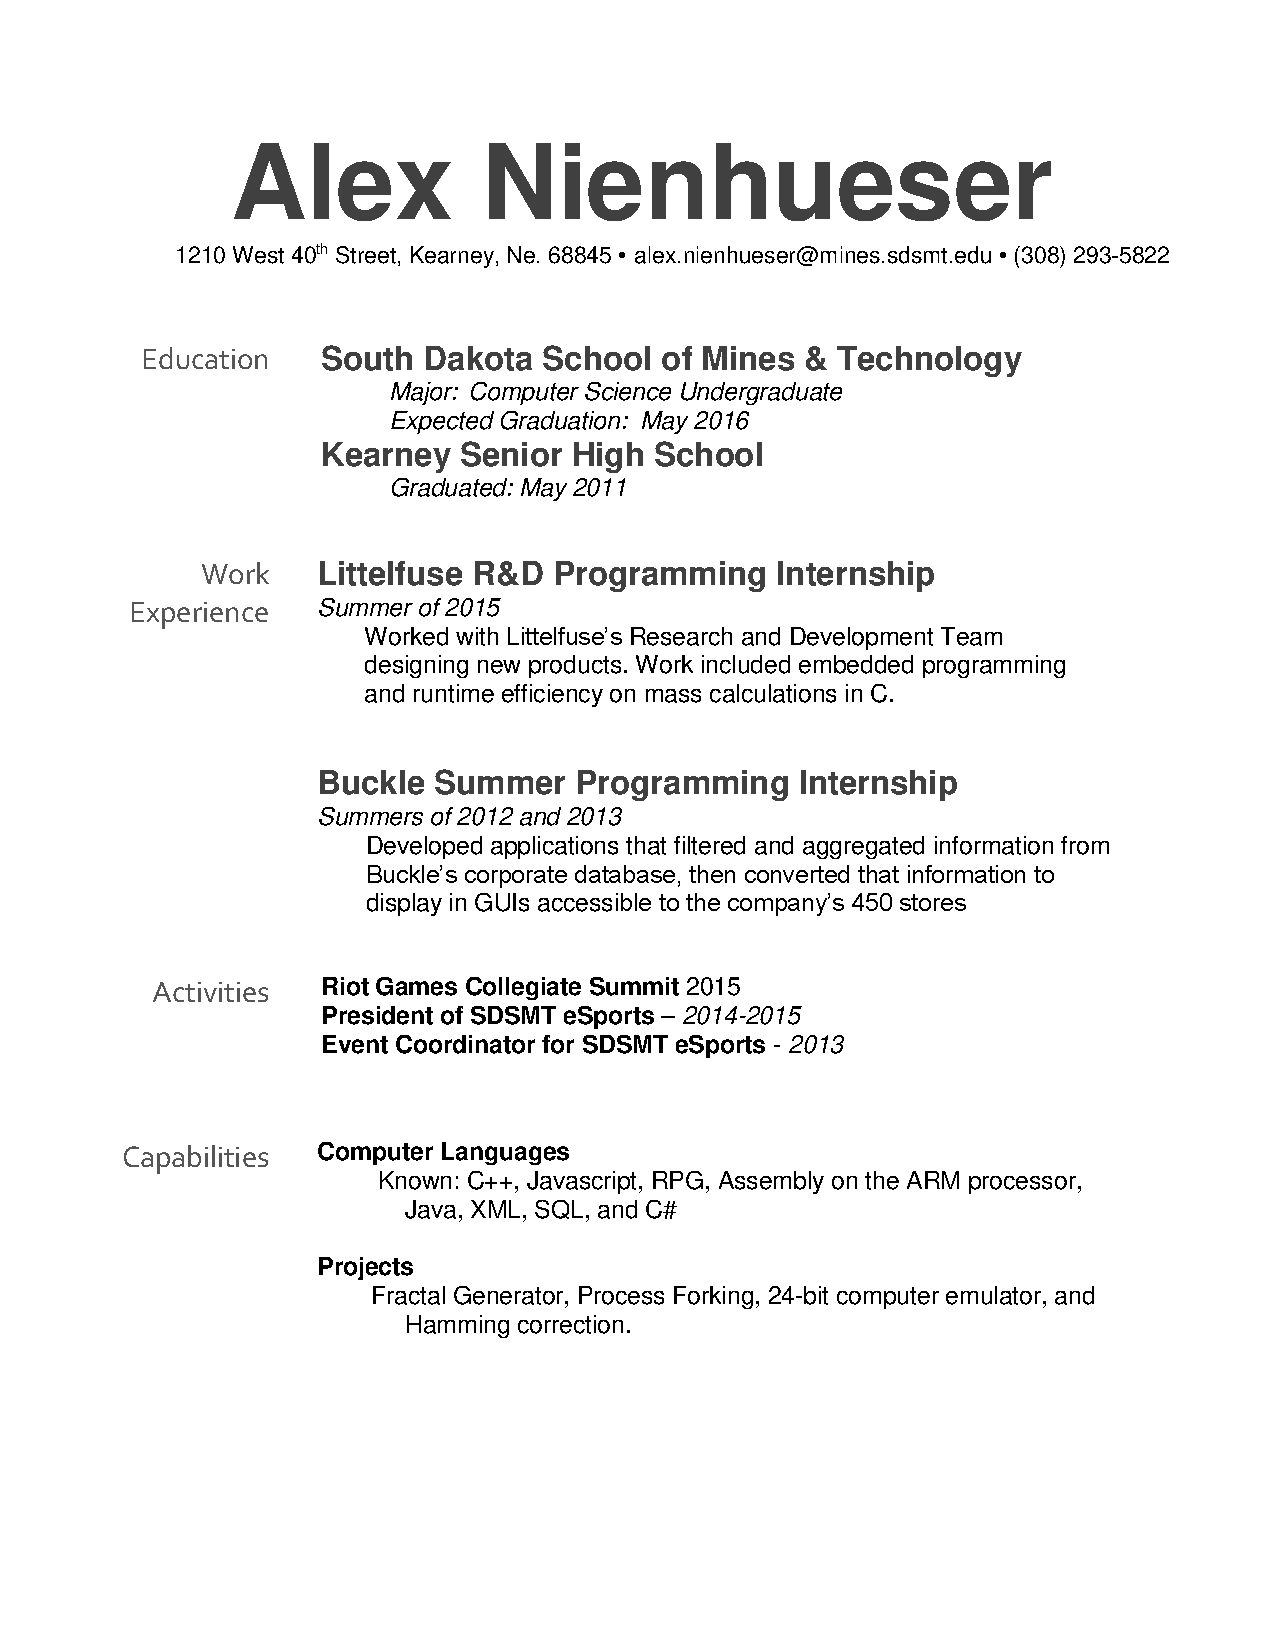
\includepdf{Resumes/Alex'sResume.pdf}
%     \includepdf{resume3.pdf}

\section{ABET:  Industrial Experience Reports}

\subsection{Mackenzie Smith}

% \includepdf{name1.pdf}

\subsection{Alex Nienhueser}

% \includepdf{name2.pdf}






\section{Client}
The Dahl Arts Center, located in downtown Rapid City South Dakota, is a huge supporter of local artists in and around the Black Hills area. 

\section{Project}
The Dahl Arts Center requests a virtual reality environment that is an accurate reflection of a current gallery in the museum.  This virtual gallery will allow a single user to experience the art pieces in a virtual environment via a virtual reality headset, in the case of this project the Oculus Rift.  Once the user has put the goggles on they will be able to choose between two movement options, free movement and on-rails which are explained further in the document.  After the movement method has been chosen, the user will explore the gallery at their discretion.  At a few selected paintings, text descriptions will be available that will pop up next to the corresponding painting allowing the user to read an interpretive description written by the artist.  There will also be some video recordings depicting the artist's methods.  Finally, the user will able to change the environment itself from the gallery to another scene to be determined. 

\subsection{Purpose of the System}
The purpose of the virtual gallery is give options people who are unable to travel to the Dahl Arts Center. By creating a virtual reality environment of one of the galleries it allows for users to enjoy the Dahl from their own home. 


\section{Business Need}
%Use this section to define what business need exist and how this software will 
%meet and/or exceed that business need.  
A museum is generally a place you physically travel to in order to experience it.  In order to experience the museum, you'll need to either walk or drive there which isn't possible for a large amount of people.  They might be disabled, lack the funds for transportation, or any other reason that prevents them from visiting the museum.  That's where this project will come in; by making the museum a piece of software, it will be easily transportable, apart from the hardware required to run it.  This will allow the Dahl to effectively take the museum out to those who might not be able to experience it otherwise.

\section{Deliverables}

The deliverables for this project will include:
\begin{description}
\item[Unreal Blueprints] \hfill \\
	These constitute the "code" for the project, which handles all of the user movement and animations in the gallery.  These will be needed if the Dahl decides to continue the project any further.

\item[Unreal Assets] \hfill \\
	The Unreal assets are the "physical" objects in the gallery.  These include the walls, paintings, alternate environment, etc...  These will be delivered as texture files, object files, and other file formats required for the Unreal Engine.
	
\item[User Documentation] \hfill \\
	This document will detail how to install, and operate the software developed during this project, as well as how to install and operate the Oculus Rift.

\item[Standalone Executable] \hfill \\
	This will be the project itself that will be able to be ran as a program on any computer that has the requisite software installed; e.g. the Oculus Rift drivers.
\end{description}   

\section{System Description}

\subsection{Unreal Engine 4.0}
This was the main development environment used during the development of the project.  It encompassed the peripheral integration as well as the visual scripting software (Blueprints).

\subsection{Oculus Rift}
The Oculus Rift SDK2 was the virtual reality headset that was used for implementing the VR in the Unreal Engine.  This component includes the headset as well as the software drivers necessary to run it.

\subsection{Xbox Controller}
This component is simply a wired Xbox 360 controller that was used to control user movement. 

\section{System Overview and Diagram}
Provide a more detailed description of the major system components
without getting too detailed.  This section should contain a
high-level block and/or flow diagram of the system highlighting the
major components.  See Figure~\ref{systemdiagram}.  This is a floating
figure environment.  \LaTeX\ will try to put it close to where it was
typeset but will not allow the figure to be split if moving it can not
happen.  Figures, tables, algorithms and many other floating
environments are automatically numbered and placed in the appropriate
type of table of contents.  You can move these and the numbers will
update correctly.

\begin{figure}[tbh]
\begin{center}
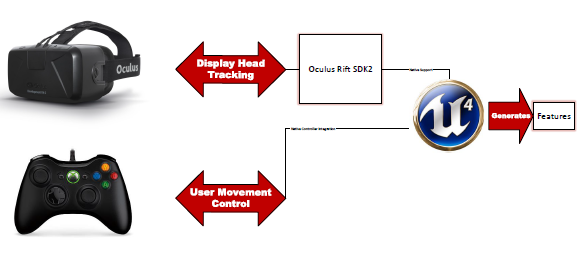
\includegraphics[width=0.75\textwidth]{Diagrams/SystemDiagram.png}
\end{center}
\caption{The overall system diagram. \label{systemdiagram}}
\end{figure}

\section{Technologies Overview}
\begin{description}
\item[Unreal Engine] \hfill \\
	The Unreal Engine was the main development environment for this project.  It had all of the facilities for integrating the movement controls, Oculus Rift, as well as the Blueprint IDE.  This technology was used to create the entire project aside from the actual paintings.  Epic Games' documentation for the Unreal Engine is very extensive and can be found here: \href{https://docs.unrealengine.com/latest/INT/}{Unreal Engine Documentation}
	
\item[Oculus Rift] \hfill \\
	The Oculus Rift was the headset used for the virtual reality implementation.  It has separate software and drivers that need to be installed before it could be used in conjunction with the Unreal Engine.  Once the drivers were installed, it can integrate seamlessly with the Engine.  Documentation on the Oculus can be found here:\href{https://developer.oculus.com/documentation/intro-vr/latest/concepts/bp_app_imaging/}{Oculus Documentation}.  Their documentation details developer best practices, which the design team implemented with the movement methods.
	
\item[Xbox Controller] \hfill \\
	The Xbox 360 controller along with any other gamepad can be integrated directly with the Unreal Engine.  This allowed the design team to simply plug the controller in and use it right away.  There is no reference material for the Xbox controller specifically, refer to Unreal Engine documentation for controller details.
\end{description}



